\documentclass{standalone}
\usepackage{thumbpdf}
\usepackage{amsfonts,amstext,amsmath,amssymb,amsthm}
\usepackage{accents}
\usepackage{color}
\usepackage{rotating}
\usepackage{verbatim}
\usepackage[utf8]{inputenc}
\usepackage{booktabs}
\usepackage{tikz}
\input{../defs}
\usepackage{tikz}

\usetikzlibrary{positioning, calc, shapes.geometric, shapes.multipart,
  shapes, arrows.meta, arrows, quotes,
  decorations.markings, external, trees}
\tikzstyle{line} = [draw, -latex']
\tikzstyle{Arrow} = [
        thick,
        decoration={
                markings,
                mark=at position 1 with {
                        \arrow[thick]{latex}
} },
        shorten >= 3pt, preaction = {decorate}
        ]

\begin{document}
\tikzset{every picture/.style={line width=0.75pt}} %set default line width to 0.75pt

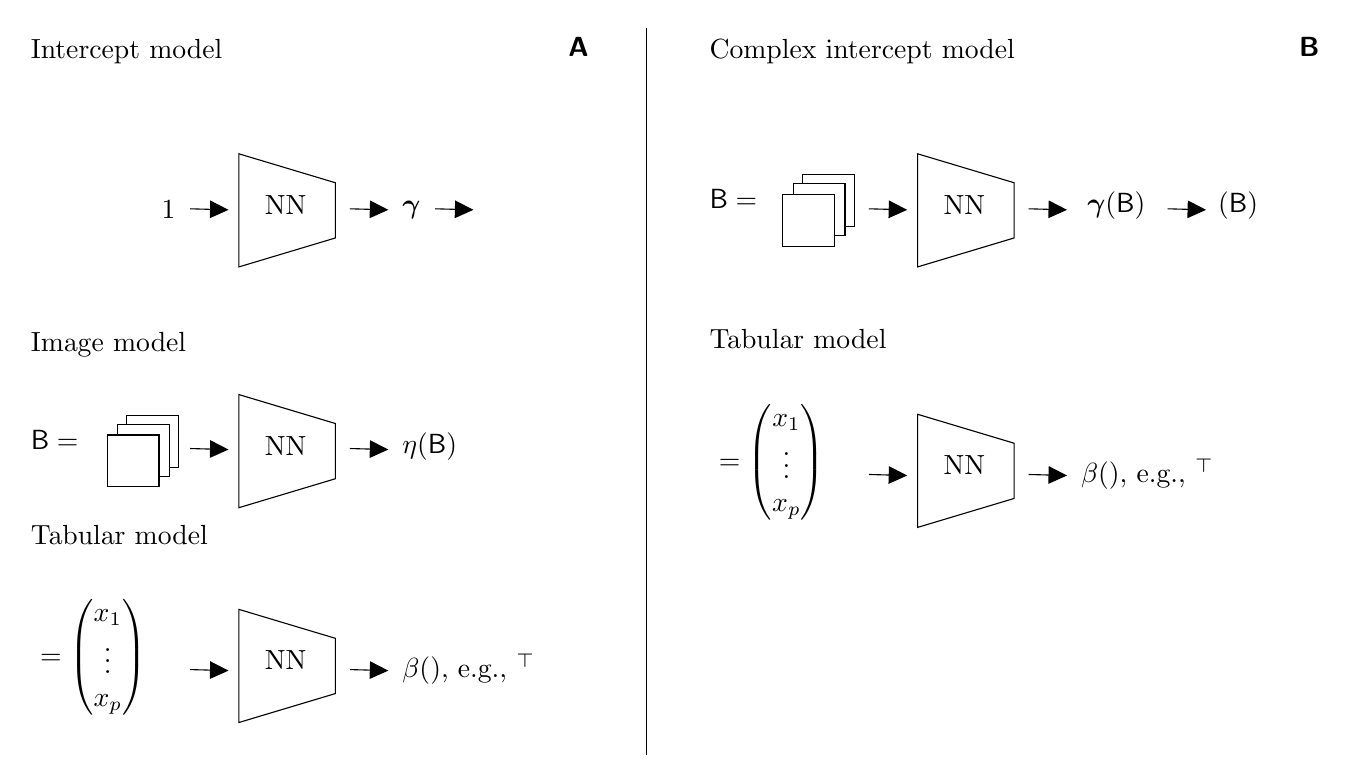
\begin{tikzpicture}[x=0.75pt,y=0.75pt,yscale=-1,xscale=1]
%uncomment if require: \path (0,372); %set diagram left start at 0, and has height of 372

%Shape: Rectangle [id:dp3625695197409119]
\draw  [fill={rgb, 255:red, 255; green, 255; blue, 255 }  ,fill opacity=1 ] (59.5,196.5) -- (84.5,196.5) -- (84.5,221.5) -- (59.5,221.5) -- cycle ;
%Shape: Rectangle [id:dp11726591920364882]
\draw  [fill={rgb, 255:red, 255; green, 255; blue, 255 }  ,fill opacity=1 ] (55,201) -- (80,201) -- (80,226) -- (55,226) -- cycle ;
%Shape: Rectangle [id:dp3338869206102766]
\draw  [fill={rgb, 255:red, 255; green, 255; blue, 255 }  ,fill opacity=1 ] (50,206) -- (75,206) -- (75,231) -- (50,231) -- cycle ;
%Shape: Trapezoid [id:dp925292527363788]
\draw   (113.5,70.5) -- (160,84.45) -- (160,111.05) -- (113.5,125) -- cycle ;
%Shape: Trapezoid [id:dp25347535714192515]
\draw   (113.5,186.5) -- (160,200.45) -- (160,227.05) -- (113.5,241) -- cycle ;
%Shape: Trapezoid [id:dp4474651715884931]
\draw   (113.5,290) -- (160,303.95) -- (160,330.55) -- (113.5,344.5) -- cycle ;
%Straight Lines [id:da6398990383758745]
\draw    (90,97) -- (105.5,97.42) ;
\draw [shift={(108.5,97.5)}, rotate = 181.55] [fill={rgb, 255:red, 0; green, 0; blue, 0 }  ][line width=0.08]  [draw opacity=0] (8.93,-4.29) -- (0,0) -- (8.93,4.29) -- cycle    ;
%Straight Lines [id:da8003507215306843]
\draw    (90,212.5) -- (105.5,212.92) ;
\draw [shift={(108.5,213)}, rotate = 181.55] [fill={rgb, 255:red, 0; green, 0; blue, 0 }  ][line width=0.08]  [draw opacity=0] (8.93,-4.29) -- (0,0) -- (8.93,4.29) -- cycle    ;
%Straight Lines [id:da8127939092483699]
\draw    (90,319) -- (105.5,319.42) ;
\draw [shift={(108.5,319.5)}, rotate = 181.55] [fill={rgb, 255:red, 0; green, 0; blue, 0 }  ][line width=0.08]  [draw opacity=0] (8.93,-4.29) -- (0,0) -- (8.93,4.29) -- cycle    ;
%Straight Lines [id:da03603117979045356]
\draw    (167,97) -- (182.5,97.42) ;
\draw [shift={(185.5,97.5)}, rotate = 181.55] [fill={rgb, 255:red, 0; green, 0; blue, 0 }  ][line width=0.08]  [draw opacity=0] (8.93,-4.29) -- (0,0) -- (8.93,4.29) -- cycle    ;
%Straight Lines [id:da0532924219005928]
\draw    (167,212.5) -- (182.5,212.92) ;
\draw [shift={(185.5,213)}, rotate = 181.55] [fill={rgb, 255:red, 0; green, 0; blue, 0 }  ][line width=0.08]  [draw opacity=0] (8.93,-4.29) -- (0,0) -- (8.93,4.29) -- cycle    ;
%Straight Lines [id:da34775465220676194]
\draw    (167,319) -- (182.5,319.42) ;
\draw [shift={(185.5,319.5)}, rotate = 181.55] [fill={rgb, 255:red, 0; green, 0; blue, 0 }  ][line width=0.08]  [draw opacity=0] (8.93,-4.29) -- (0,0) -- (8.93,4.29) -- cycle    ;
%Straight Lines [id:da4008660940208326]
\draw    (208,97) -- (223.5,97.42) ;
\draw [shift={(226.5,97.5)}, rotate = 181.55] [fill={rgb, 255:red, 0; green, 0; blue, 0 }  ][line width=0.08]  [draw opacity=0] (8.93,-4.29) -- (0,0) -- (8.93,4.29) -- cycle    ;
%Shape: Rectangle [id:dp34930982096174523]
\draw  [fill={rgb, 255:red, 255; green, 255; blue, 255 }  ,fill opacity=1 ] (385,80.5) -- (410,80.5) -- (410,105.5) -- (385,105.5) -- cycle ;
%Shape: Rectangle [id:dp7404586976873827]
\draw  [fill={rgb, 255:red, 255; green, 255; blue, 255 }  ,fill opacity=1 ] (380.5,85) -- (405.5,85) -- (405.5,110) -- (380.5,110) -- cycle ;
%Shape: Rectangle [id:dp7373905728938016]
\draw  [fill={rgb, 255:red, 255; green, 255; blue, 255 }  ,fill opacity=1 ] (375.5,90) -- (400.5,90) -- (400.5,115) -- (375.5,115) -- cycle ;
%Shape: Trapezoid [id:dp7470580792541655]
\draw   (440.5,70.5) -- (487,84.45) -- (487,111.05) -- (440.5,125) -- cycle ;
%Shape: Trapezoid [id:dp6740979939914692]
\draw   (440.5,196) -- (487,209.95) -- (487,236.55) -- (440.5,250.5) -- cycle ;
%Straight Lines [id:da01800918830200926]
\draw    (417,97) -- (432.5,97.42) ;
\draw [shift={(435.5,97.5)}, rotate = 181.55] [fill={rgb, 255:red, 0; green, 0; blue, 0 }  ][line width=0.08]  [draw opacity=0] (8.93,-4.29) -- (0,0) -- (8.93,4.29) -- cycle    ;
%Straight Lines [id:da1189432563199535]
\draw    (417,225) -- (432.5,225.42) ;
\draw [shift={(435.5,225.5)}, rotate = 181.55] [fill={rgb, 255:red, 0; green, 0; blue, 0 }  ][line width=0.08]  [draw opacity=0] (8.93,-4.29) -- (0,0) -- (8.93,4.29) -- cycle    ;
%Straight Lines [id:da5655996514004799]
\draw    (494,97) -- (509.5,97.42) ;
\draw [shift={(512.5,97.5)}, rotate = 181.55] [fill={rgb, 255:red, 0; green, 0; blue, 0 }  ][line width=0.08]  [draw opacity=0] (8.93,-4.29) -- (0,0) -- (8.93,4.29) -- cycle    ;
%Straight Lines [id:da6503778171820888]
\draw    (494,225) -- (509.5,225.42) ;
\draw [shift={(512.5,225.5)}, rotate = 181.55] [fill={rgb, 255:red, 0; green, 0; blue, 0 }  ][line width=0.08]  [draw opacity=0] (8.93,-4.29) -- (0,0) -- (8.93,4.29) -- cycle    ;
%Straight Lines [id:da4528412503300122]
\draw    (561,97) -- (576.5,97.42) ;
\draw [shift={(579.5,97.5)}, rotate = 181.55] [fill={rgb, 255:red, 0; green, 0; blue, 0 }  ][line width=0.08]  [draw opacity=0] (8.93,-4.29) -- (0,0) -- (8.93,4.29) -- cycle    ;
%Straight Lines [id:da14228788553774474]
\draw    (310,10) -- (310,360) ;

% Text Node
\draw (12,14) node [anchor=north west][inner sep=0.75pt]   [align=left] {Intercept model};
% Text Node
\draw (12,155) node [anchor=north west][inner sep=0.75pt]   [align=left] {Image model};
% Text Node
\draw (12,248) node [anchor=north west][inner sep=0.75pt]   [align=left] {Tabular model};
% Text Node
\draw (75,92) node [anchor=north west][inner sep=0.75pt]    {$1$};
% Text Node
\draw (12,202.4) node [anchor=north west][inner sep=0.75pt]    {$\mathsf{B} =$};
% Text Node
\draw (12,283.4) node [anchor=north west][inner sep=0.75pt]    {$\rx \ =\begin{pmatrix}
x_{1}\\
\vdots \\
x_{p}
\end{pmatrix}$};
% Text Node
\draw (124.75,89.25) node [anchor=north west][inner sep=0.75pt]   [align=left] {NN};
% Text Node
\draw (124.75,205.25) node [anchor=north west][inner sep=0.75pt]   [align=left] {NN};
% Text Node
\draw (124.75,308.75) node [anchor=north west][inner sep=0.75pt]   [align=left] {NN};
% Text Node
\draw (191,203.4) node [anchor=north west][inner sep=0.75pt]    {$\eta (\mathsf{B})$};
% Text Node
\draw (191,310.4) node [anchor=north west][inner sep=0.75pt]    {$\beta (\rx)$, e.g., $\rx^{\top }\shiftparm$};
% Text Node
\draw (191,92) node [anchor=north west][inner sep=0.75pt]    {$\boldsymbol{\gamma}$};
% Text Node
\draw (231,92) node [anchor=north west][inner sep=0.75pt]    {$\parm$};
% Text Node
\draw (339,14) node [anchor=north west][inner sep=0.75pt]   [align=left] {Complex intercept model};
% Text Node
\draw (339,154) node [anchor=north west][inner sep=0.75pt]   [align=left] {Tabular model};
% Text Node
\draw (339,86.4) node [anchor=north west][inner sep=0.75pt]    {$\mathsf{B} =$};
% Text Node
\draw (339,189.4) node [anchor=north west][inner sep=0.75pt]    {$\rx \ =\begin{pmatrix}
x_{1}\\
\vdots \\
x_{p}
\end{pmatrix}$};
% Text Node
\draw (451.75,89.25) node [anchor=north west][inner sep=0.75pt]   [align=left] {NN};
% Text Node
\draw (451.75,214.75) node [anchor=north west][inner sep=0.75pt]   [align=left] {NN};
% Text Node
\draw (518,216.4) node [anchor=north west][inner sep=0.75pt]    {$\beta (\rx)$, e.g., $\rx^{\top }\shiftparm$};
% Text Node
\draw (521,87.4) node [anchor=north west][inner sep=0.75pt]    {$\boldsymbol{\gamma}(\mathsf{B})$};
% Text Node
\draw (584,87.4) node [anchor=north west][inner sep=0.75pt]    {$\parm(\mathsf{B})$};
% Text Node
\draw (271,13) node [anchor=north west][inner sep=0.75pt]   [align=left] {\textbf{\textsf{A}}};
% Text Node
\draw (623,13) node [anchor=north west][inner sep=0.75pt]   [align=left] {\textbf{\textsf{B}}};
\end{tikzpicture}
\end{document}
